\documentclass[useAMS, usenatbib, preprint, 12pt]{aastex}
\usepackage{cite,natbib}
\usepackage{epsfig}
\usepackage{cases}
\usepackage[section]{placeins}
\usepackage{graphicx, subfigure}
\usepackage{color}

\title{Systematics-insensitive periodic signal search with K2}

\begin{document}

\newcommand{\oxford}{1}
\newcommand{\nyu}{2}
\newcommand{\cfa}{3}

\author{%
   Ruth Angus\altaffilmark{\oxford},
   Daniel Foreman-Mackey\altaffilmark{\nyu},
   John A. Johnson\altaffilmark{\cfa},
   {\it et al.}
}

\altaffiltext{\oxford}{Subdepartment of Astrophysics, University of Oxford, OX1 3RH, UK}
\altaffiltext{\nyu}{Center for Cosmology and Particle Physics, New York University, NY, USA}
\altaffiltext{\cfa}{Harvard-Smithsonian Center for Astrophysics, 60 Garden St.,
Cambridge, MA, USA}

\begin{abstract}

% Aims
From pulsating stars to transiting exoplanets, the search for periodic signals
in {\it K2} data is relevent to a long list of scientific goals.
Systematics affecting {\it K2} light curves due to the decreased
space craft pointing precision inhibit the easy extraction of periodic signals
from the data.
We here develop a method for producing periodograms of K2 light curves that
are insensitive to pointing-induced systematics.
% Methods
Sine-fitting periodograms use a generative model to find the frequency
of the sine wave that best describes the data.
We extend this principle by including systematic trends in our generative
model as well as a sum of sine and cosine functions over a grid of
frequencies.
% Results
Using this method we are able to produce periodograms, free from
systematic features.
The quality of the resulting periodograms are such that we can recover
acoustic oscillations in giants and detect variable stars, eclipsing binaries
and exoplanet candidates without the need for any detrending.
% Whilst this method performs extremely well in the high part of frequency space,
% relevent for giant asteroseismology, it is not optimised for measuring stellar
% rotation periods.
This method performs well for signals with periods from 1 hour up to 2 days,
however it is not optimized for periods much greater than 5 days.
This is due to the fact that some common trends between stars vary on
timescales similar to rotation periods.

\end{abstract}

\section{Introduction}
\label{Introduction}

After the failure of {\it Kepler}'s third reaction wheel, the spacecraft was
repurposed, and the {\it K2} mission began in 2014.
The excellent precision achieved by the original {\it Kepler} mission relied
on extremely precise pointing, for which three reaction wheels were required.
After the failure of one of these wheels, the {\it Kepler} team devise a new
pointing scheme where the spacecraft is stabilised by the Solar wind, so long
as it points at fields in the ecliptic plane.
% With just two reaction wheels it is still possible to maintain relatively
% precise pointing by using the Solar wind to stabilise the space craft and only
% observing ecliptic fields.
In this configuration the spacecraft is able to maintain an unstable
equilibrium, with the two reaction wheels controlling pitch and yaw whilst the
spacecraft slowly rolls about the boresight.
The spacecraft fires its thrusters once every $\sim$ 6 hours to correct for
this slow drift.
As stars move across pixels with different sensitivities, rtheir flux varies.
Developing methods for the extraction of information from K2 light
curves, despite the reduced pointing precision, is therefore extremely
important.
Several methods for detrending {\it K2} light curves have already been
developed: \citet{Vanderburg2014} and \citet{Crossfield2015} use simple
aperture photometry and correct the light curve of each star individually.
\citet{Aigrain2015} use a Gaussian process to model the non-linear dependence
of stellar flux on the roll angle of the telescope.
Whilst these methods are successful at removing most systematic trends and
produce light curves suitable for exoplanet search and some stellar
variability studies, any signal still remaining due to the 6 hour thruster
fires is detremental to asteroseismology.
A detrending method for {\it K2} light curves, specifically intended for the
asteroseismic analysis of giant stars is being developed by Lund {\it et al.}
(in prep.) in which the systematics due to roll are corrected, again on
a star-by-star basis and any remaining periodic signals at 47 $\mu$Hz (6 hour
period) or its harmonics are removed by prewhitening.
The method developed here, the Systematics-Insenstive Periodogram (SIP)
produces a periodogram of the data without the need for detrending or
prewhitening.

The {\it Kepler} spacecraft is currently observing its 4th field and data for
campaigns 0 and 1 have been released.
Within each field there are thousands of variable, rotating, and pulsating
stars as well as exoplanet hosts.
The original {\it Kepler} mission provided a huge set of light curves with
periodic behaviour on timescales ranging from a few minutes to a few months.
Many fields were enormously advanced (asteroseismology in particular) by its
excellent precision.
Fundamental stellar parameters---in some cases, extremely precise ones---can
be calculated for {\it Kepler} asteroseismic stars from the power spectra of
their light curves.
% Around 600 Solar-like oscillators, pulsating at $\sim$5 minute to
% $\sim$hour-long timescales, were observed in short cadence mode.
Although Sun-like stars oscillate at high frequencies and require
short-cadence observations, pulsations of giant stars lie below the Nyquist
frequency set by the 28.5 minute sampling rate of long cadence {\it Kepler}
data: 283 $\mu$Hz.
% The Fast Fourier Transform (FFT) and sine-fitting periodogram are fundamental
% tools in the asteroseismic toolbox.
Asteroseismic analysis of data from the original {\it Kepler} mission is
traditionally conducted upon detrended light curves.
For short cadence {\it Kepler} data, this detrending method is described in
\citet{Garcia2011}.
Figure \ref{fig:raw} demonstrates the need for careful systematics treatment
of {\it K2} photometry for asteroseismology.
The top panel shows a Lomb-Scargle periodogram of the raw, simple aperture
photometry\footnote{The method used to extract this photometry is described in
\textsection \ref{sec:Method}} of EPIC 201183188, a pulsating giant star.
The large peaks at $\sim$ 47 $\mu$Hz and its harmonics are caused by the
regular thruster fires of the spacecraft.
The bottom panel shows the Lomb-Scargle periodogram of this light curve, after
it has been detrended using the method of \citet{Vanderburg2014}.
The large peaks are still present in the detrended light curve.

Active regions on the surface of rotating stars produce periodic variations
in flux and stellar rotation periods can therefore be measured from
{\it Kepler} light curves.
Stellar rotation is a field of active interest as the rotation period of star
can be used to infer its age \citep{Skumanich1972, Barnes2007, Epstein2014},
is thought to be tied to the stellar magnetic dynamo, and could even reveal
dynamical interations with companion stars or planets \citep[e.g.][]{Beky2014,
Poppenhaeger2014}.
% Rotation periods are also useful for {\it Kepler} exoplanet characterization.
% Active regions can produce variability in radial velocity as well as
% photometry and can masquerade as planetary signals.
% It is therefore extremely useful to be able measure the rotation period of the
% star directly from the light curve.
Current methods for measuring rotation periods from {\it Kepler} light curves
include periodogram \citep[e.g.][]{Reinhold2013}, AutoCorrelation Function
(ACF) \citep{McQuillan2013} and wavelet \citep[e.g.][]{Garcia2014} analysis,
or some combination thereof.
Stellar variability is not typically sinusoidal, therefore sine-fitting
periodograms are not perfectly suited for measuring rotation periods.
For this reason, the ACF method is often favoured over the periodogram method.
However, because autocorrelation is performed on the data, and is not
a generative model, we cannot use autocorrelation techniques on non-detrended
{\it K2} data.
A quasi-periodic Gaussian process is a much better effective model for stellar
variability than a sinusoid, however we are not only concerned with stellar
rotation so choose to focus on the more generally applicable (and
computationally tractable) sine-wave periodogram, leaving the Gaussian process
for future consideration.

Aside from asteroseismology and stellar rotation there are many other fields
of research, targeted by {\it K2}, that utilize periodic information.
These include searching for eclipsing binaries, variable stars and exoplanets,
and even studying white dwarfs and AGN.
The development of tools for extracting periodic information from {\it K2}
data is essential if it is to be as revolutionary in time-domain
astronomy as the original {\it Kepler} mission was.

\section{Method}
\label{sec:Method}

The method implemented in this paper is an extention of the planet-search
algorithm developed by \citet{Foreman-Mackey2015} (hereafter FM15).
All targets observed by {\it Kepler} move on the CCD in the same way and
therefore the systematics affecting each individual star's light curve have
shared properties.
The FM12 method utilizes this fact and decomposes the trends into a set of
`Eigen Light Curves' (ELCs) using Principle Component Analysis (PCA).
This method is similar to that used to produce PDC-MAP data for the original
{\it Kepler} mission \citep[][]{Stumpe2012, Smith2012}.
The resulting ELCs can then be used to model any campaign 1 {\it K2} light
curve, and specifically, can model the data in conjunction with an arbitrary
physical model.  FM15 downloaded the target pixel files for all stars observed
in campaign 1; 21,703 in total.
The position of each star was predicted using the world coordinate system and
10 circular apertures placed around the star with radii varying from 1 to
5 pixels in steps of 0.5 pixels.
Following the procedure of \citet{Vanderburg2014}, the aperture producing the
light curve with the lowest CDPP within a 6 hour window
\citet{Christiansen2012} was selected\footnote{The simple aperture photometry
light curves for campaigns 0 and 1 are available at
http://bbq.dfm.io/ketu/lightcurves/}.
PCA was then performed on the full set of targets in order to produce ELCs.
FM15 used 150 of these ELCs with a transit model in order to
search for exoplanet candidates without the need for a `detrending' step.
The likelihood of the data, conditioned on the ELC-plus-transit
model was calculated over a fine grid of periods and transit depths, resulting
in the detection of 36 new exoplanet candidates.
We use exactly the same technique to find periodic signals in {\it K2} data,
however, instead of a transit, our model is a sine wave.
This model is linear, therefore the likelihood function conditioned on
a specific frequency can be calculated and the systematics model marginalized
over analytically.

Following the notation in FM15, our model for the $k$th star can be written
\begin{equation}
	\mathbf{f_k} = \mathbf{A}\mathbf{w_k} + \mathrm{noise},
\end{equation}
where $\mathbf{f_k}$ is the vector of $N$ flux values,
\begin{equation}
	\mathbf{f_k} = (f_{k,1}, f_{k,2}, f_{k,3}, ..., f_{k,N})^T
\end{equation}
at times
\begin{equation}
	\mathbf{t_k} = (t_1, t_2, t_3, ..., t_N)^T.
\end{equation}
$\mathbf{A}$ is the design matrix:
\begin{eqnarray}
	\mathbf{A} &=& \left (\begin{array}{ccccccc}
	x_{1,1} & x_{2,1} & \cdots & x_{150,1} & 1 & \sin(2\pi\nu t_1) & \cos(2\pi\nu t_1) \\
	x_{1,2} & x_{2,2} & \cdots & x_{150,2} & 1 & \sin(2\pi\nu t_2) & \cos(2\pi\nu t_2\\
    && \vdots &&&\\
	x_{1,N} & x_{2,N} & \cdots & x_{150,N} & 1 & \sin(2\pi\nu t_N) & \cos(2\pi\nu t_N)
\end{array}\right )
\end{eqnarray}
where the $x_{ij}$s are the ELCs\footnote{Campaign 0 and 1 ELCs are
available at http://bbq.dfm.io/ketu/elcs/}, with $i$ denoting the ELC number
and $j$ the time index. The maximum likelihood solution for the weight vector,
$\mathbf{w}$ is
\begin{equation}
	\mathbf{w_k}^* \gets (\mathbf{A}^T\mathbf{A})^{-1}\mathbf{A}^T\mathbf{f_k} \end{equation}
and the sum of the last two elements of $\mathbf{w}_k$, squared, provides the
power of the signal at a given frequency.
This operation is performed over a grid of frequencies to produce a power
spectrum.
We then calculate the signal-to-noise ratio (S/N) frequency by comparing the
power at each frequency to a robust estimate of the variance in power across
all frequencies.
In practise, we use the S/N, rather than power to produce a
periodogram\footnote{The code used in this project can be found at
https://github.com/RuthAngus/K2rotation.}.

\subsection{Injections}

In order to test the sensitivity and completeness of the SIP method,
we injected sinusoids into real {\it K2} light curves.
EPIC 201311941 was identified as a quiet star with no significant periodic
variability at any frequency.
10,000 sinusoids with periods between 1 to 50 days and amplitudes ranging from
1 to 1000 parts-per-million (ppm) (linearly in log-space) were injected into
the raw campaign 1 light curve of EPIC 201311941.
The highest peak in the resulting periodogram of each light curve was recorded.
If the period of the highest peak lay within 10\% of the true period, this was
considered a successful detection.
This procedure was repeated for periods ranging from 1 hour to 2 days in order
test the recovery of signals at frequencies relevent to asteroseismology.
The resulting completeness maps are shown in figures \ref{fig:K2_hist_r} and
\ref{fig:K2_hist_a}.
The SIP is uniformly sensitive across all frequencies relevant to giant
asteroseismology.
Using the SIP we are able to recover signals with amplitudes of a few ppm.
One caveat of this test, however, is that a single sine wave with a constant
amplitude over the full 80 day baseline of campaign 1 may not necessarily be
a realistic model of acoustic modes in giant stars and is certainly not
representative of stellar variability.
Real signals, therefore are likely to be less easy to detect.
Figure \ref{fig:K2_hist_a} shows the lower sensitivity of the SIP for periods
greater than $\sim$ 2 days.

\section{Results and discussion}
\subsection{Application to asteroseismology}

An example Lomb-Scargle periodogram\footnote{All Lomb-Scargle periodograms
produced in this project were calculated using the gatspy Python module:
https://github.com/astroML/gatspy/tree/master/gatspy/periodic}
of the raw {\it K2 photometry} for EPIC 201211472 is shown in figure
\ref{fig:raw}.
Peaks appearing at 47 $\mu$Hz and its harmonics are produced by the regular
$\sim$ 6 hour thruster fires that repoint the spacecraft.
These peaks are also present in periodograms of the \citet{Vanderburg2014}
detrended light curves.
The presence of systematic signals at these timescales are problematic for
asteroseismic analysis since they lie in a region of frequency space
that is often populated by giant asteroseismic modes.
It is possible to remove these signals by `prewhitening' the data, i.e.
subtracting a sine wave of that frequency from the data, however this process
will artificially supress all signals, both systematic and astrophysical, at
that frequency.
No such procedure is necessary for our method.

We selected long cadence targets from the GO1059 proposal: "Galactic
Archaeology on a grand scale" (PI: Stello, D.) in order to test the SIP.
SIPs of the raw data were produced by calculating the signal to noise
ratio of the amplitudes of single sine and cosine functions, plus 150 ELCs
conditioned on the data at a range of frequencies.
In order to identify asteroseismic oscillation modes, we searched for a power
excess in the SIPs using the method of \citet{Huber2009}.
Autocorrelation functions are calculated for sections of the power spectrum in
order to search for regions of increased correlation and locate the frequency
of maximum power.
The increased correlation arises from the even frequency spacing of acoustic
modes, and the frequency of maximum correlation at the location of the power
excess corresponds to the large frequecy separation, $\Delta\nu$.
Figures \ref{fig:1} to \ref{fig:6} show example power spectra of 6 targets for
which we detect pulsations using this method.

% Our method does not perfectly model the systematics for every star.
% Of the power spectra generated for each of the n stars in GO1049, n of them
% showed power at 47$\mu$Hz.
% Examples of power spectra containing residual systematic features are shown in
% figure ?.

We also applied our analysis to 3 red giants and 3 $\delta$ Scuti stars
identified by Lund {\it et al.} (in prep), in campaign 0.
Since campaign 0 was shorter, $\sim$ 25 days, the SIP method is not as
successful at modelling the systematics as for campaign 1.
% and fewer stars observed?
For this reason the 47$\mu$Hz peaks caused by the regular 6 hour thruster
firings appear, with relatively high amplitudes for 2 of the 6 targets and with
moderate amplitudes for another 2 of the 6.
The two most sucessful SIPs, for targets EPIC 202086286 and EPIC
202068435 are shown in figure \ref{fig:c0}.

\subsection{Application to stellar rotation}
The top panel of figure \ref{fig:rotation_poster_child} shows the light curve
of an active, rotating star, EP201317002.
This light curve has been detrended using the method of
\citet{Vanderburg2014}.
The middle and bottom panels show an ACF and Lomb-Scargle periodogram of the
detrended light curve.
The highest peaks in both the ACF and periodogram are located at around 10
days.
Figure \ref{fig:K2_rotation_poster_child} shows the raw light curve of the
same target (top panel) with its SIP, calculated by modeling the data as
a linear combination of ELCs and a sine and cosine function at a range of
frequencies (bottom panel).
Each of these 3 methods measures a rotation period of around 10 days for this
target.
Figure \ref{fig:top5} shows the 5 ELCs with the highest weights for this star.
Most of these ELCs vary on timescales close to 10 days.
The light curve of EPIC 201317002 is therefore easily described by the ELCs
alone, without the need for an additional sinusoidal signal.
In fact, many of the ELCs have dominant sinusoidal variation, with periods
of a few days (the cause of this is still unclear).
For this reason the SIP method is not as well suited to stellar rotation as it
is to asteroseismology, which is concerned with much higher frequency signals.

\subsection{Further examples}
Figures \ref{fig:RRLyrae} and \ref{fig:EB} show the conditioned light curves
and SIPs of an RR Lyrae star, selected from Guest observing program GO1018 and
an Eclipsing Binary (EB), selected from the {\it K2} EB and variable star
catalogue of \citet{Armstrong2015}, respectively.
Figure \ref{fig:planet} shows the conditioned light curve and SIP of a
short-period planet candidate.
This planet has a period of around 0.4 days, short enough to be detectable
with a periodogram, as was demonstrated for a number of ultra-short
period {\it Kepler} exoplanets by \citet{Sanchis-Ojeda2014}.
The top panels of these three figures show the {\it K2} light curves of these
objects, conditioned on the highest amplitude sinusoidal signal in the
periodograms.

Photometric variability in dwarf stars on timescales less than 8 hours, often
known as flicker, has been linked to surface gravity, g
\citep[][]{Bastien2013, Kipping2014}.
The metrics used to quantify photometric variability include finding the range
in intensity, counting the number of zero crossings and calculating the
root-mean-square (RMS) of the light curve.
Although these features are related to signal processing, they are operations
performed on detrended light curves, not inferred from periodograms.
However, it may be possible to derive a property of the periodogram that scales
with the density or surface gravity of a star, for example, the mean excess
power at frequencies near those relevent to granulation timescales.

\section{Conclusions}
We demonstrate that modelling campaign 1 {\it K2} photometry as a linear
combination of 150 PCA components plus a sinusoid can produce beautiful
periodograms without the need for detrending.
We find that the 47 $\mu$Hz signal, generated by the space craft thruster
fires is not present in the vast majority of systematics-insensitive
periodograms for more than 4000 targets
selected from the {\it K2} guest observer program, GO1059, "Galactic
Archaeology on a grand scale" (PI: Stello, D.).
The SIP method is highly successful for campaign 1 targets where the large
number of stars, observed for a baseline of 80 days ensures that most of the
systematics are captured in the ELCs and we anticipate that is will
be equally effective for the up-and-coming campaigns.
It is not, however, suitable for campaign 0 light curves, where the reduced
observational baseline means that the systematics are not fully captured by the
top 150 ELCs.

The successes of the SIP method are most apparent in the high frequency regime,
particularly in the region of frequency space relevent to the study of
asteroseismic oscillations in giant stars.
The SIP method also performs well for signals with periods between $\sim$
1 hour and $\sim$ 2 days, however it is not well optimised for measuring
stellar rotation periods, due to the fact that many ELCs are dominated by
periodic variations on the same timescales as the rotation periods.

\begin{figure*}
\begin{center}
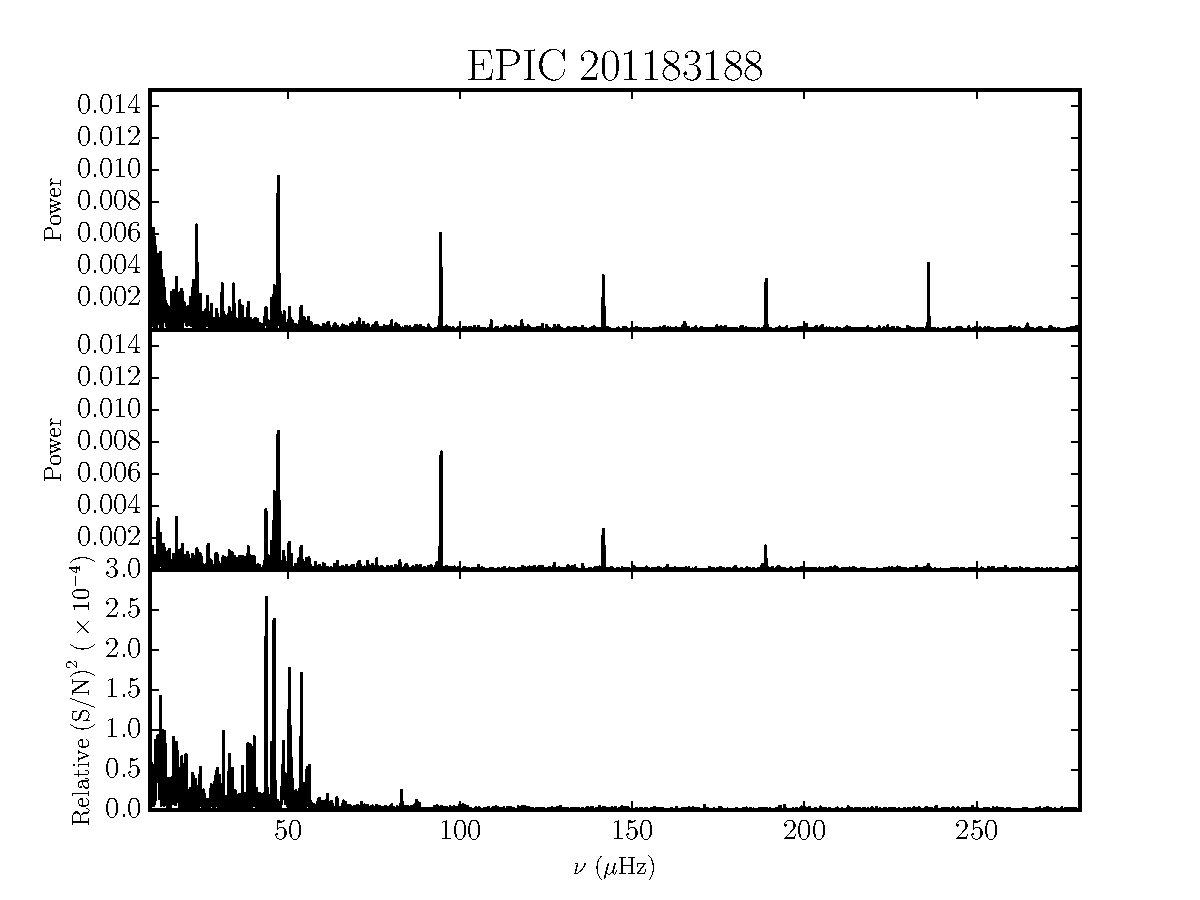
\includegraphics[width=6in, clip=true]{rawvbg_201183188.pdf}
\caption{Lomb-scargle periodogram of the raw (Top) and detrended
	 (bottom) {\it K2} photometry for EPIC 201183188. The light curve was
 	 detrended using the method of \citet{Vanderburg2014}. The peak at
	 $\sim$ 47 $\mu$Hz and its harmonics produced by the regular spacecraft
	 thruster fires are still present in periodogram of the detrended
	 data.}
\label{fig:raw}
\end{center}
\end{figure*}

\begin{figure}
\begin{center}
	\subfigure[]{
            \label{fig:1}
	    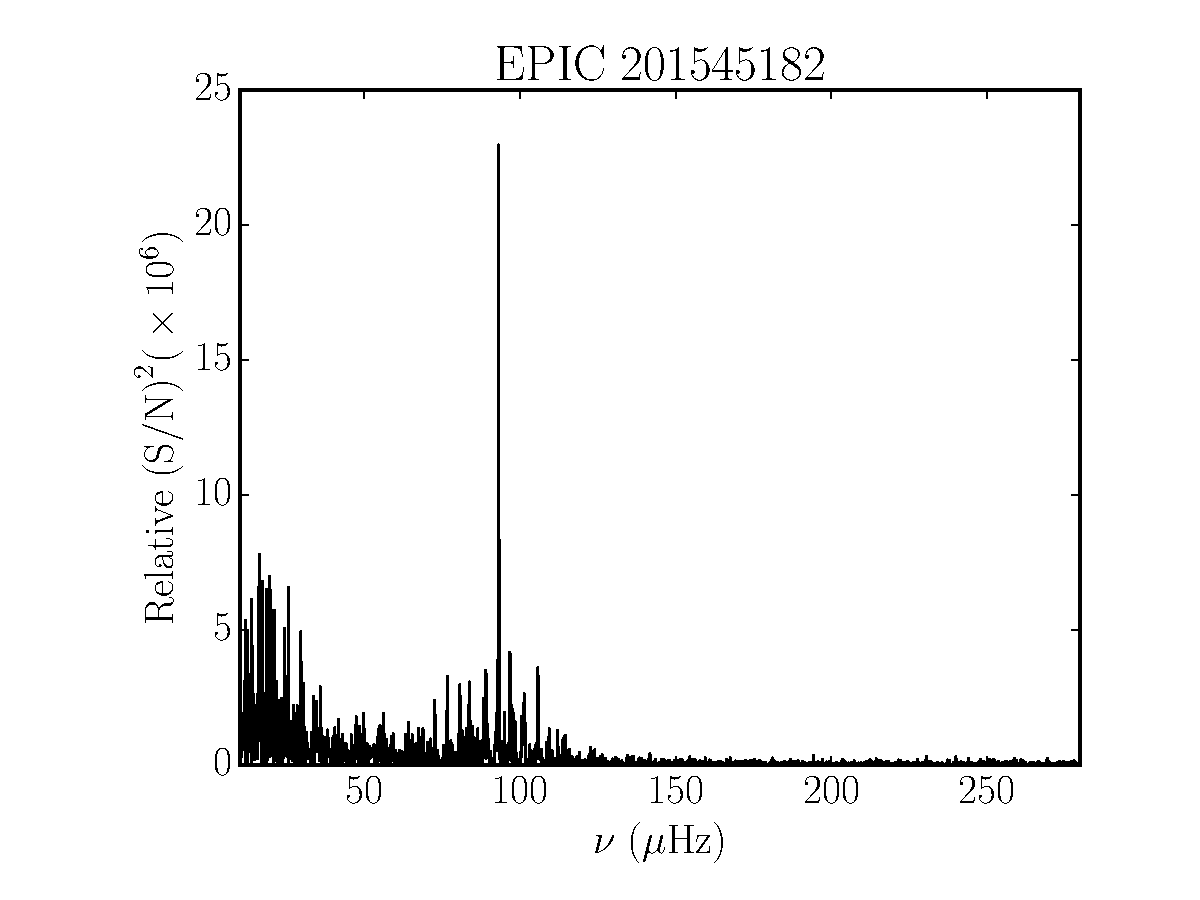
\includegraphics[width=3in]{201545182.pdf}
        }
	\subfigure[]{
            \label{fig:2}
	    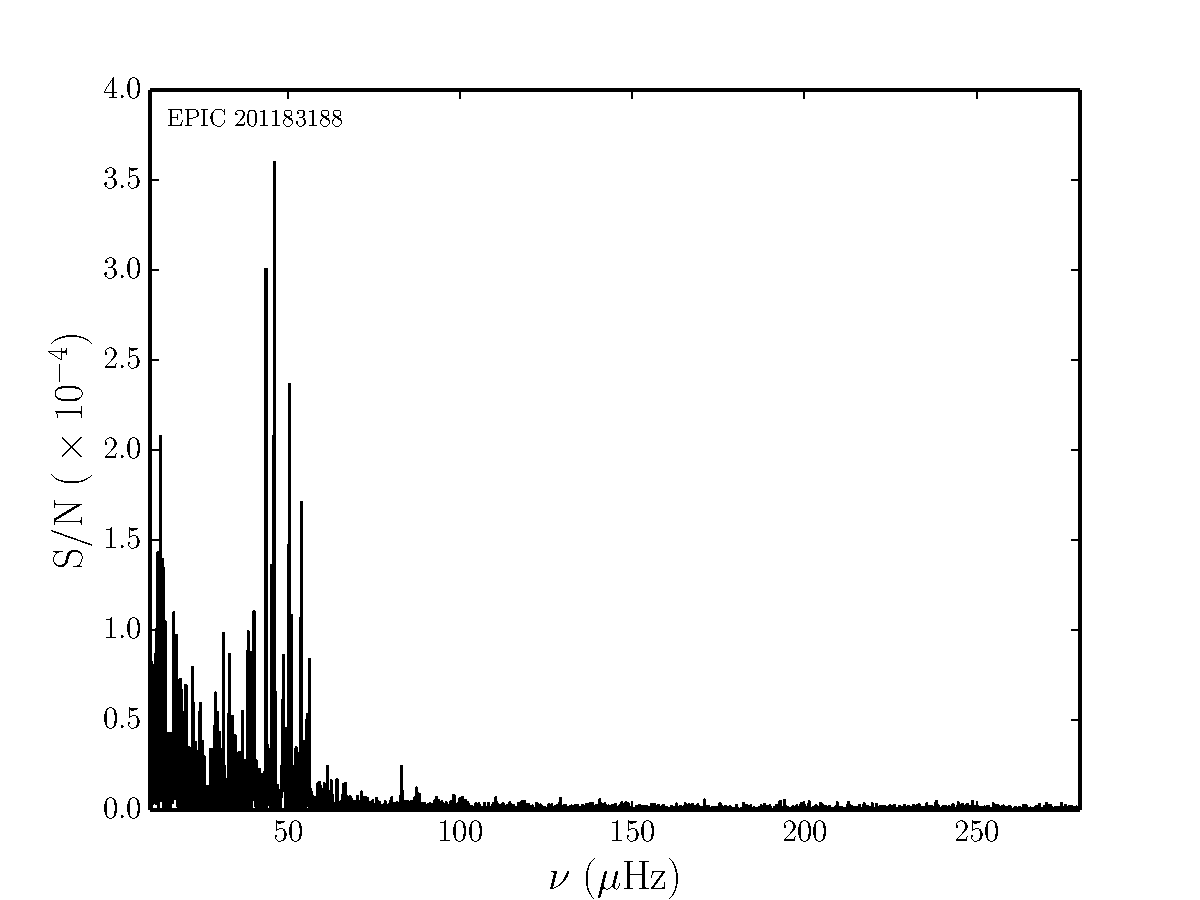
\includegraphics[width=3in]{201183188.pdf}
        }
	\subfigure[]{
            \label{fig:3}
	    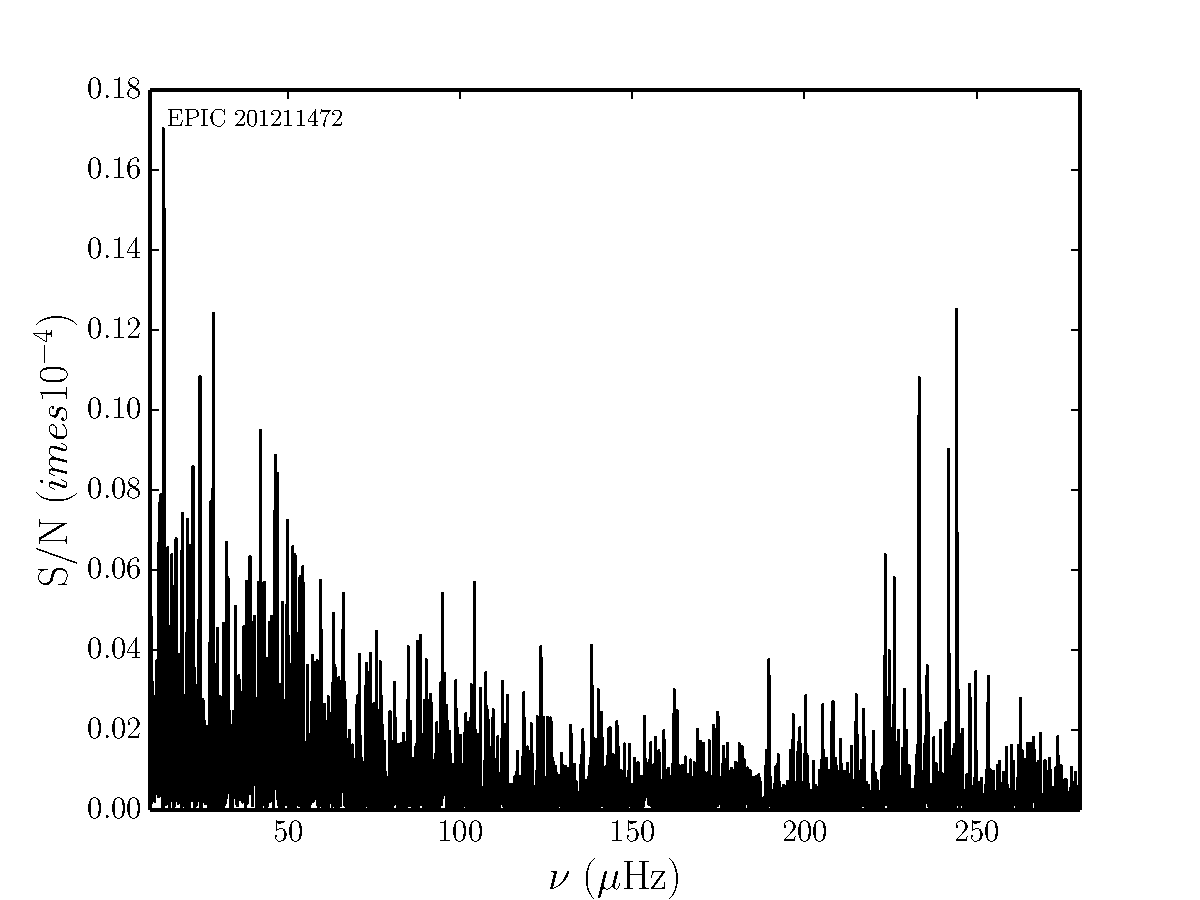
\includegraphics[width=3in]{201211472.pdf}
        }
	\subfigure[]{
            \label{fig:4}
	    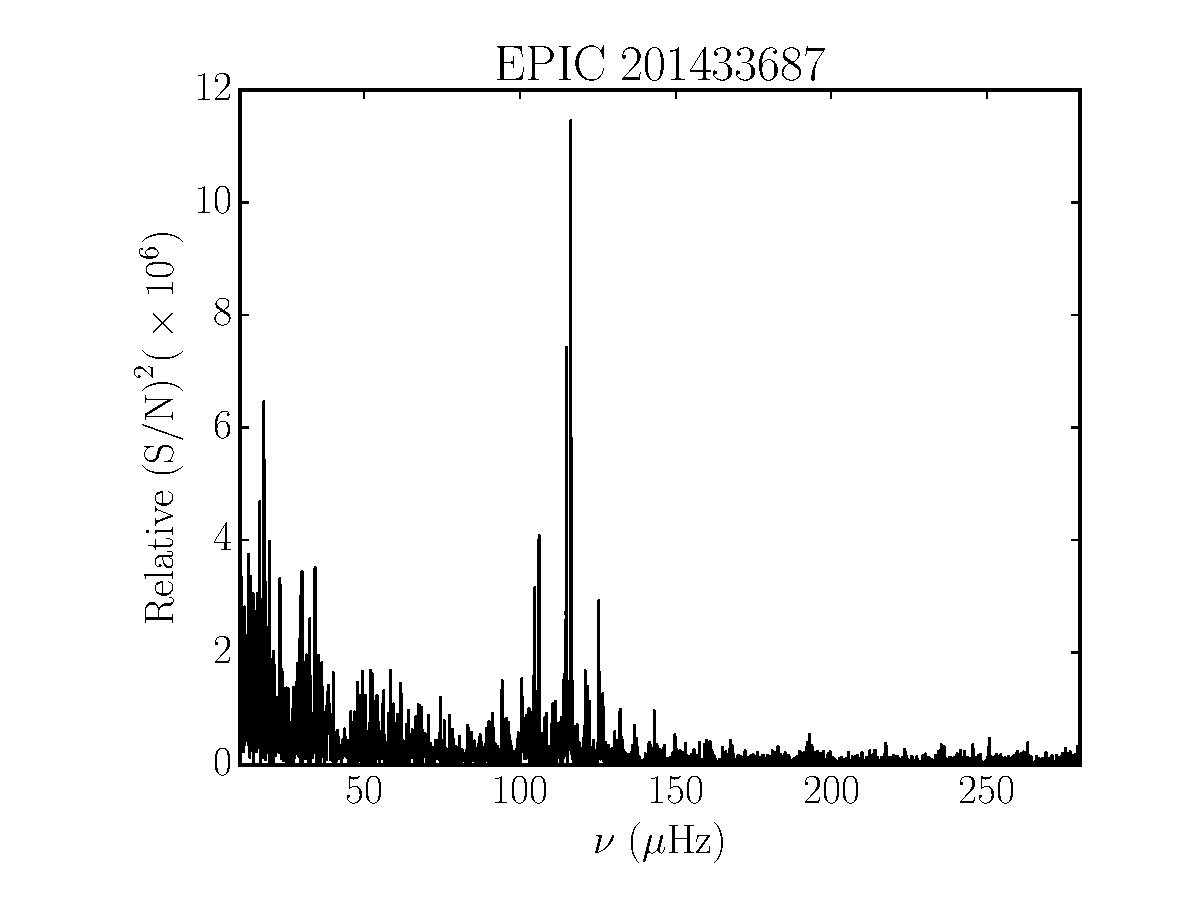
\includegraphics[width=3in]{201433687.pdf}
        }
	\subfigure[]{
            \label{fig:5}
	    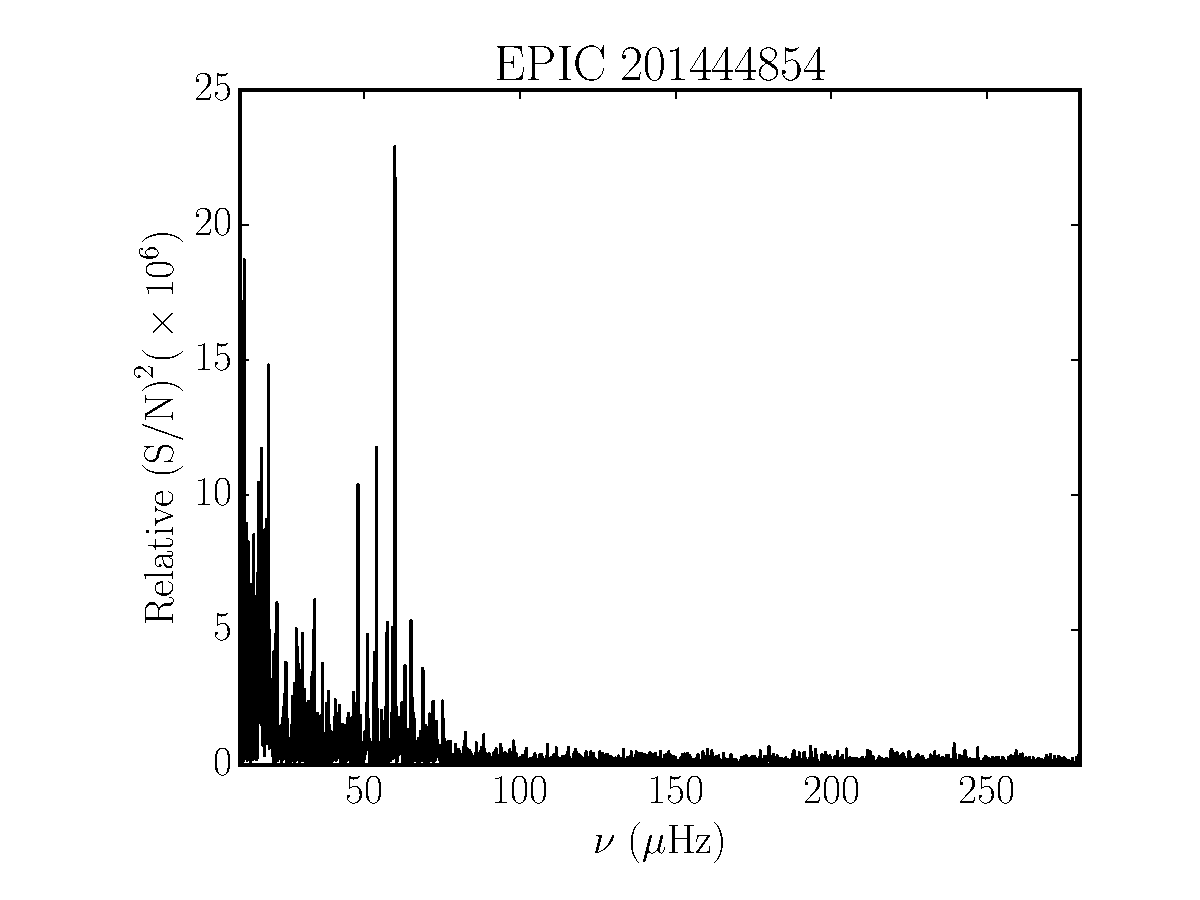
\includegraphics[width=3in]{201444854.pdf}
        }
	\subfigure[]{
            \label{fig:6}
	    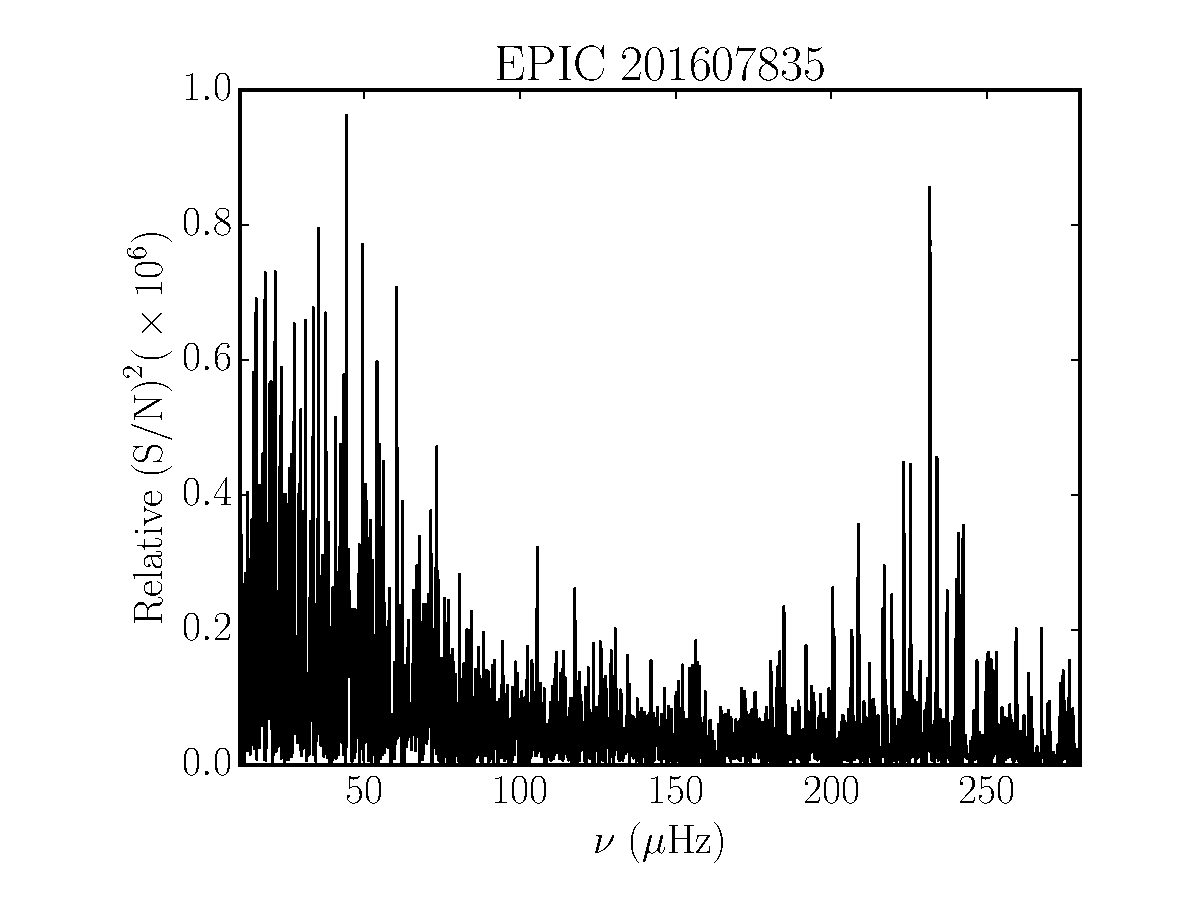
\includegraphics[width=3in]{201607835.pdf}
        }
    \end{center}
    \caption{SIPs of 6 long cadence {\it K2} giants with pulsations. These
	     were selected from the guest observing program, GO1059 and were
	     identified using the method of \citet{Huber2009}.
\label{fig:astero_examples}}
\end{figure}

\begin{figure}
\begin{center}
	\subfigure[]{
            \label{fig:c01}
	    \includegraphics[width=3in]{202086286.pdf}
        }
	\subfigure[]{
            \label{fig:c02}
	    \includegraphics[width=3in]{202068435.pdf}
        }
    \end{center}
    \caption{SIPs of 2 long cadence {\it K2} giants with
	    pulsations from campaign 0. These targets were identified as
	    pulsating giants by Lund {\it et al.} (in prep).
\label{fig:c0}}
\end{figure}

\begin{figure*}
\begin{center}
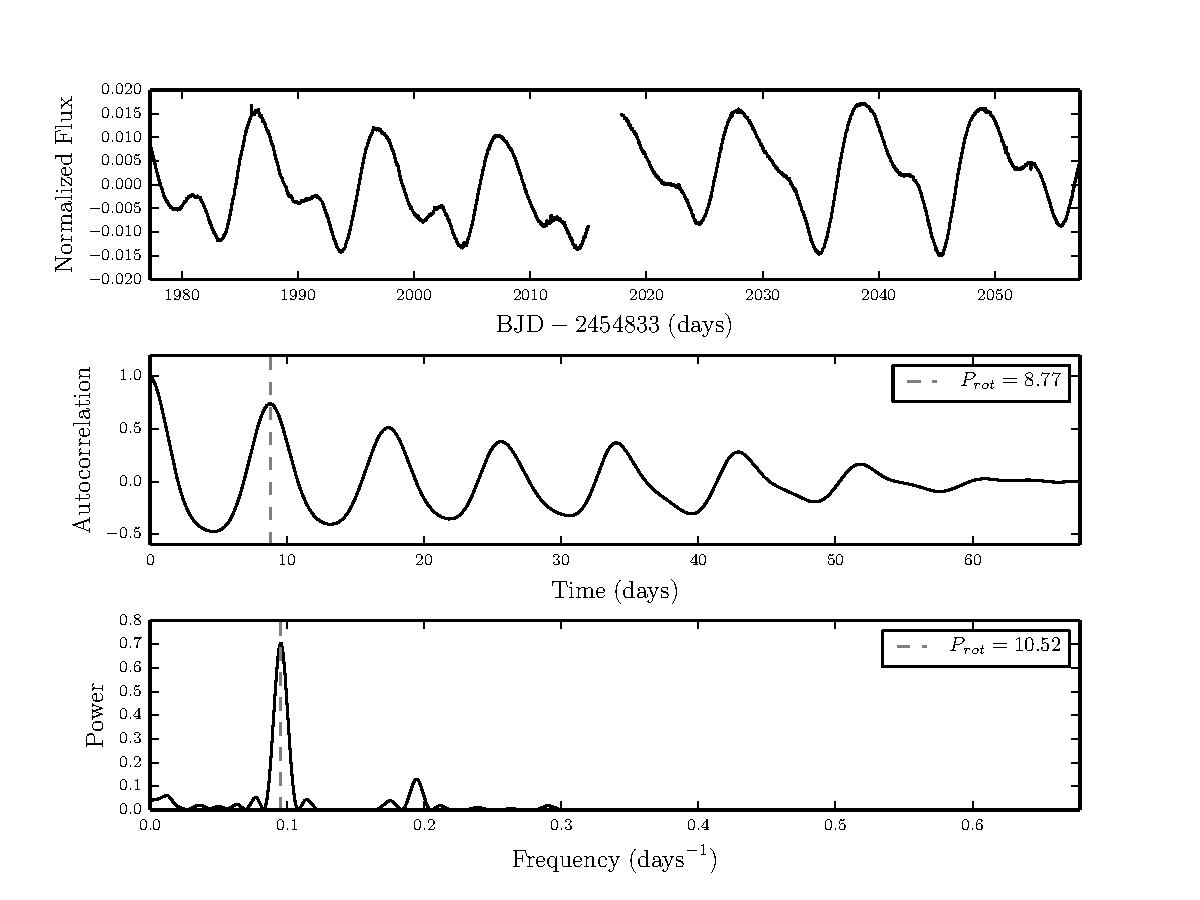
\includegraphics[width=6in, clip=true]{rotation_poster_child.pdf}
\caption{{\it Top}: Light curve of EPIC 201317002, detrended using the method
of \citet{Vanderburg2014}. {\it Middle}: Autocorrelation function of the
detrended light curve. The autocorrelation function method measures a rotation
period of 8.77 days for this star. {\it Bottom}: The Lomb-Scargle periodogram
of the detrended light curve. The highest peak in the periodogram is centred at
10.52 days.}
\label{fig:rotation_poster_child}
\end{center}
\end{figure*}

\begin{figure*}
\begin{center}
\includegraphics[width=6in, clip=true]{K2_rotation_201317002.pdf}
\caption{{\it Top}: Raw light curve of EPIC 201317002. {\it Bottom}: A
periodogram produced by modelling the data using the top 150 ELCs
plus a sine and cosine function at a range of frequencies. The highest peak in
the periodogram is centred at 10.34 days.}
\label{fig:K2_rotation_poster_child}
\end{center}
\end{figure*}

\begin{figure*}
\begin{center}
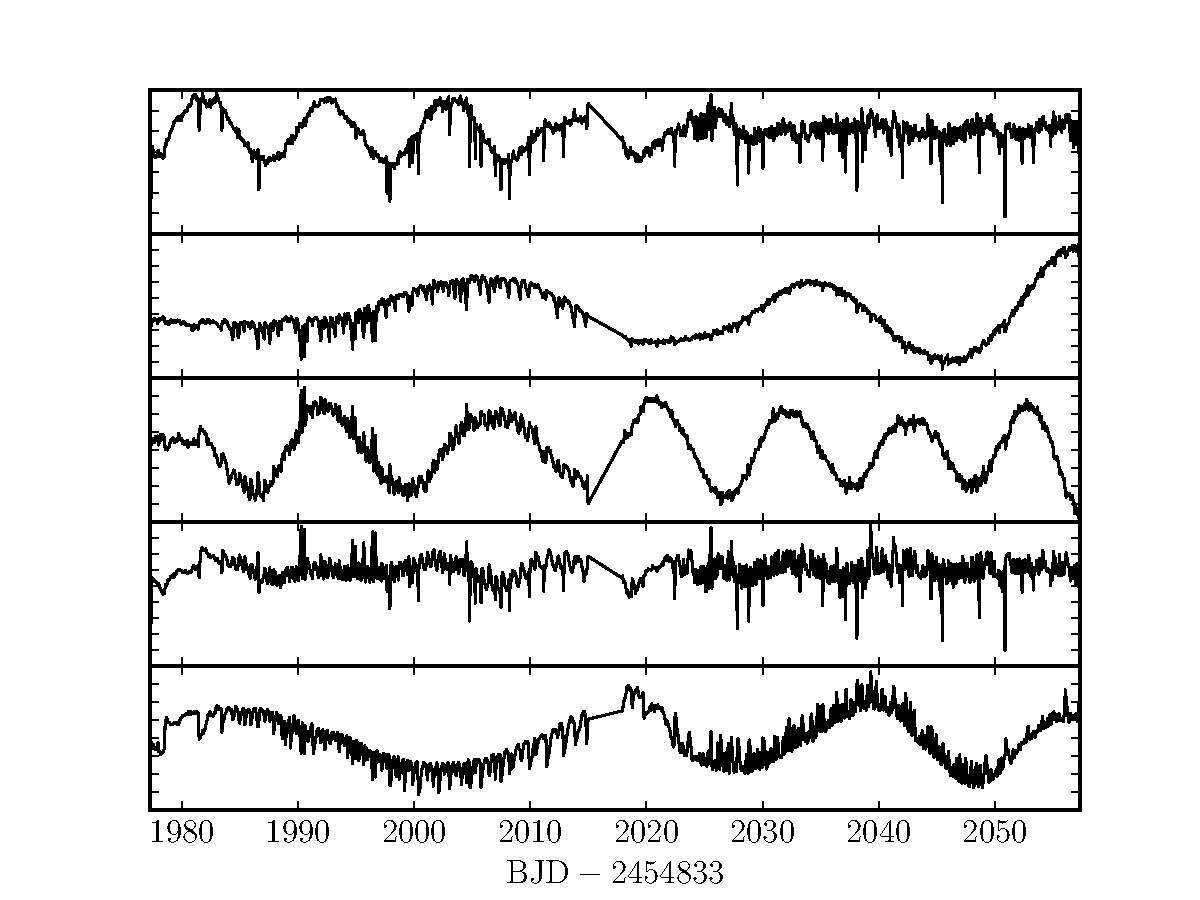
\includegraphics[width=6in, clip=true]{201317002_top5.pdf}
\caption{The 5 highest-weighted ELCs for EPIC 201317002. At least 3 of these
	ELCs show sinusoidal variability with a $\sim$ 10 day period.
	The light curve of EPIC 201317002 is therefore easily described by the
	ELCs alone, without the additional sinusoid model.
	This illustrates the difficulty in measuring rotation periods using the
	SIP method.}
\label{fig:top5}
\end{center}
\end{figure*}

\begin{figure*}
\begin{center}
\includegraphics[width=6in, clip=true]{K2_hist_r.pdf}
\caption{Completeness of sinusoidsal signal recovery. 10,000 Sinusoidal signals
with a range of periods and amplitudes were injected into the raw light curve
of the non-variable star EPIC 201311941. In the range of periods relevent to
stellar rotation ($\sim$ 1 - 60 days), we are most complete at the shortest
periods, however the SIP is not well suited to measuring long periods.}
\label{fig:K2_hist_r}
\end{center}
\end{figure*}

\begin{figure*}
\begin{center}
\includegraphics[width=6in, clip=true]{K2_hist_a.pdf}
\caption{Completeness of sinusoidsal signal recovery. 10,000 Sinusoidal signals
with a range of periods and amplitudes were injected into the raw light curve
of the non-variable star EPIC 201311941. In the range of periods relevent to
asteroseismology ($\sim$ 1 - 48 hours), we are uniformily complete down to
very low amplitudes.}
\label{fig:K2_hist_a}
\end{center}
\end{figure*}

\begin{figure*}
\begin{center}
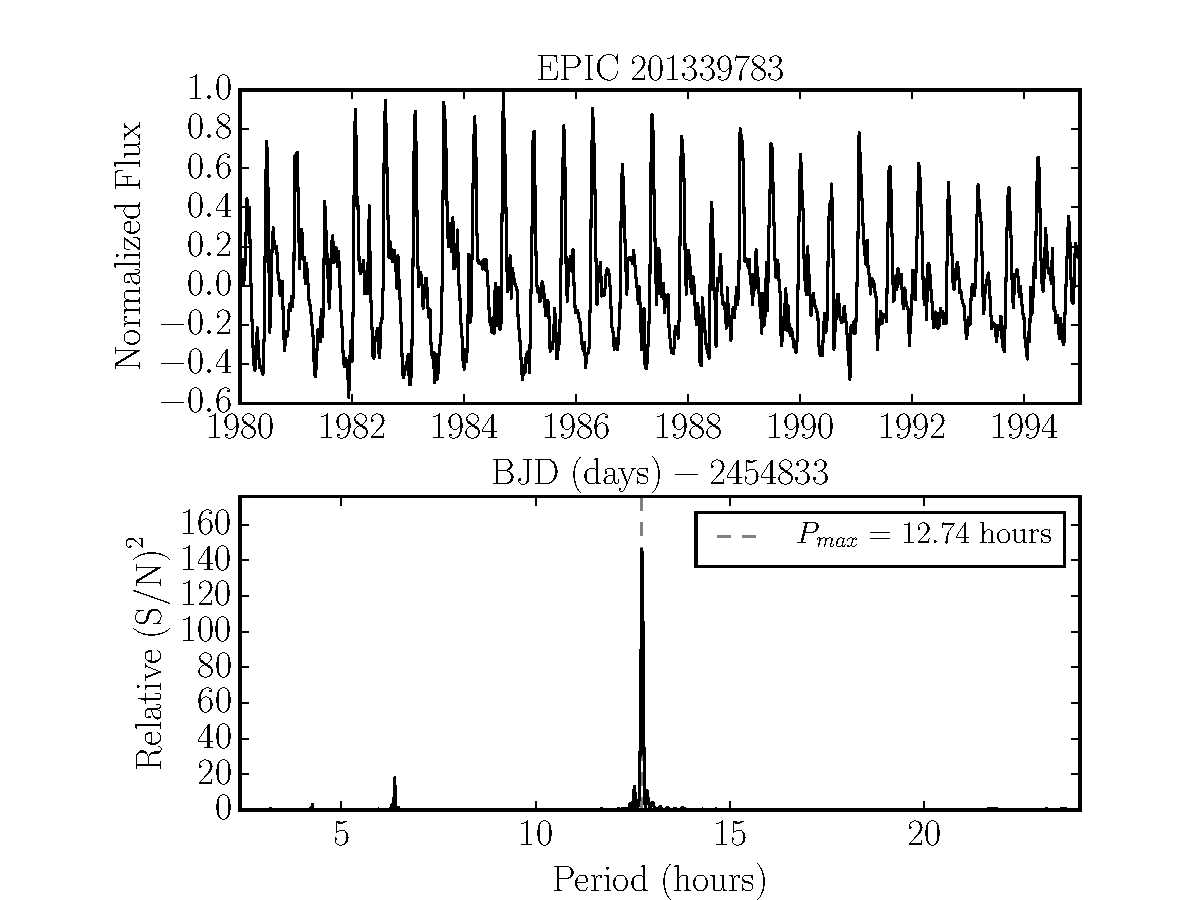
\includegraphics[width=6in, clip=true]{RR_201339783.pdf}
\caption{{\it Top:} The light curve of RR Lyrae star, EPIC 201339783,
	conditioned on the highest amplitude sinusoidal signal found in the
	SIP. {\it Bottom:} The systematic-insensitive periodogram of
	this light curve. This target was selected from GO1018.}
\label{fig:RRLyrae}
\end{center}
\end{figure*}

\begin{figure*}
\begin{center}
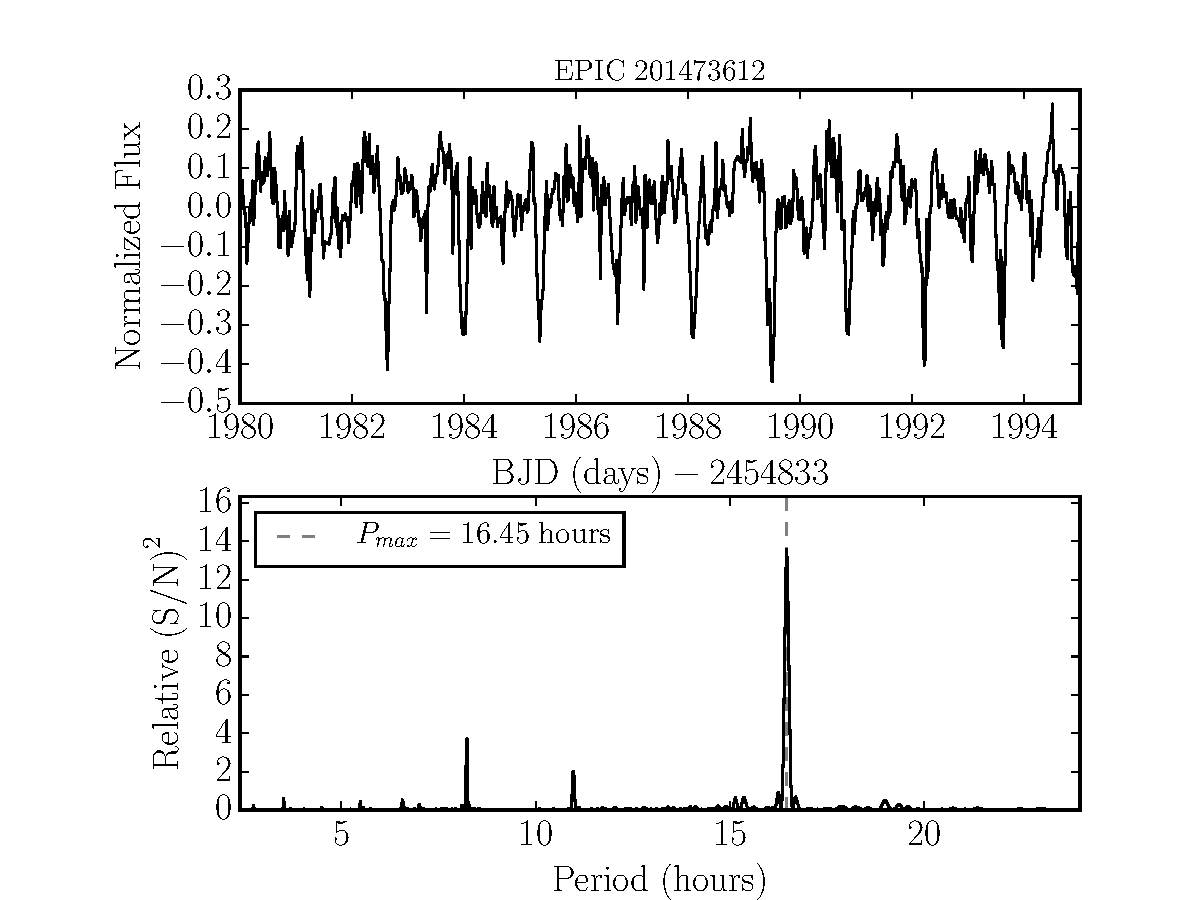
\includegraphics[width=6in, clip=true]{EB_201473612.pdf}
\caption{{\it Top:} The light curve of eclipsing binary, EPIC 201473612,
	conditioned on the highest amplitude sinusoidal signal found in the
	SIP. {\it Bottom:} The systematic-insensitive periodogram of
	this light curve. This target was selected from the catalogue of EBs
	and variable stars of \citet{Armstrong2015}.}
\label{fig:EB}
\end{center}
\end{figure*}

\begin{figure*}
\begin{center}
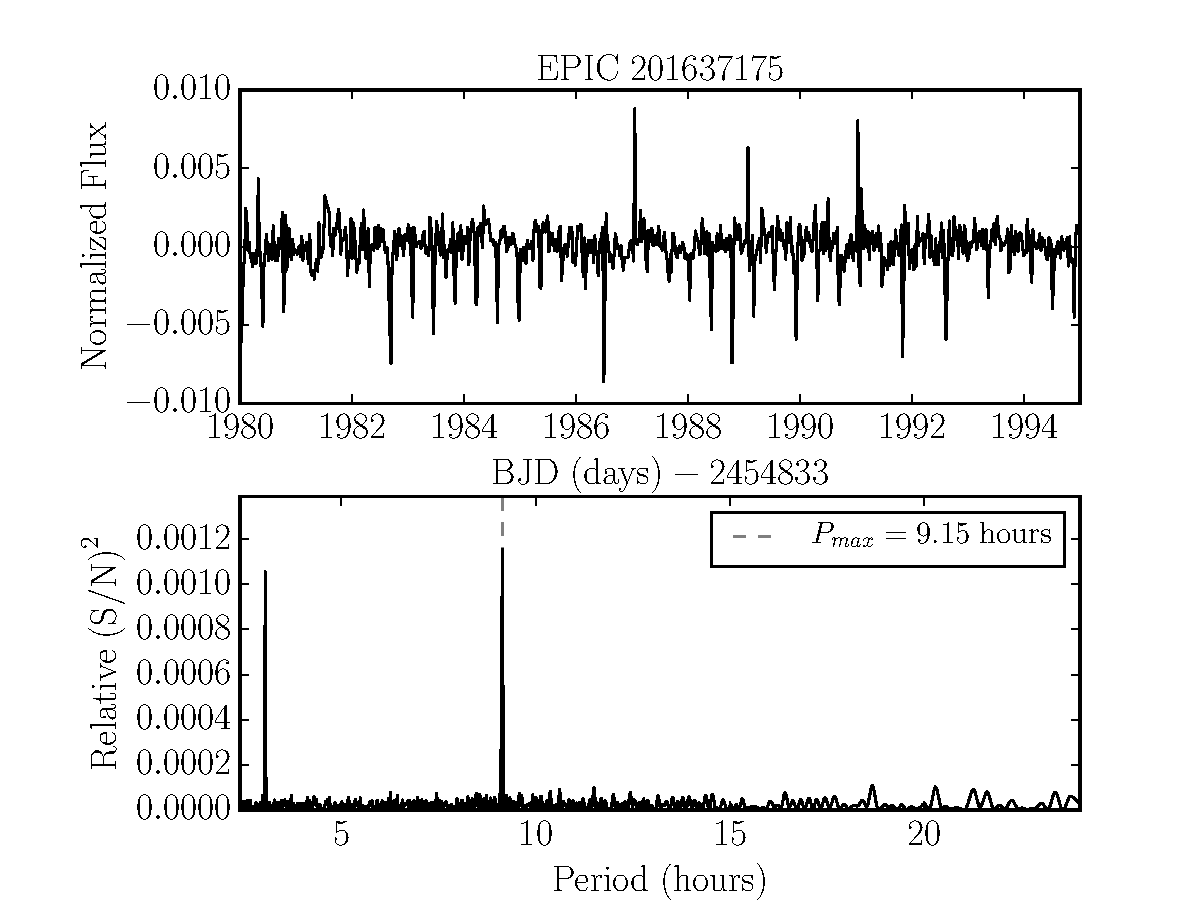
\includegraphics[width=6in, clip=true]{planet_201637175.pdf}
\caption{{\it Top:} The light curve of exoplanet candidate, EPIC 201637175,
	conditioned on the highest amplitude sinusoidal signal found in the
	periodogram. {\it Bottom:} The systematic-insensitive periodogram of
	this target.}
\label{fig:planet}
\end{center}
\end{figure*}

\bibliographystyle{plainnat}
\bibliography{k2rotation}
\end{document}
